\documentclass[tikz,border=14pt]{standalone}

\usepackage[T1]{fontenc}
\usepackage{lmodern}
\usetikzlibrary{arrows.meta,positioning,fit}

\definecolor{PrimaryRed}{HTML}{8B1E1E}
\definecolor{DeepNavy}{HTML}{15324A}
\definecolor{MidTeal}{HTML}{287D7A}
\definecolor{SoftBlue}{HTML}{DDEEFF}
\definecolor{SoftGreen}{HTML}{E4F1E8}
\definecolor{SoftGold}{HTML}{F8EDC7}
\definecolor{SoftRose}{HTML}{F5E2E7}
\definecolor{SoftGray}{HTML}{F4F4F4}

\begin{document}
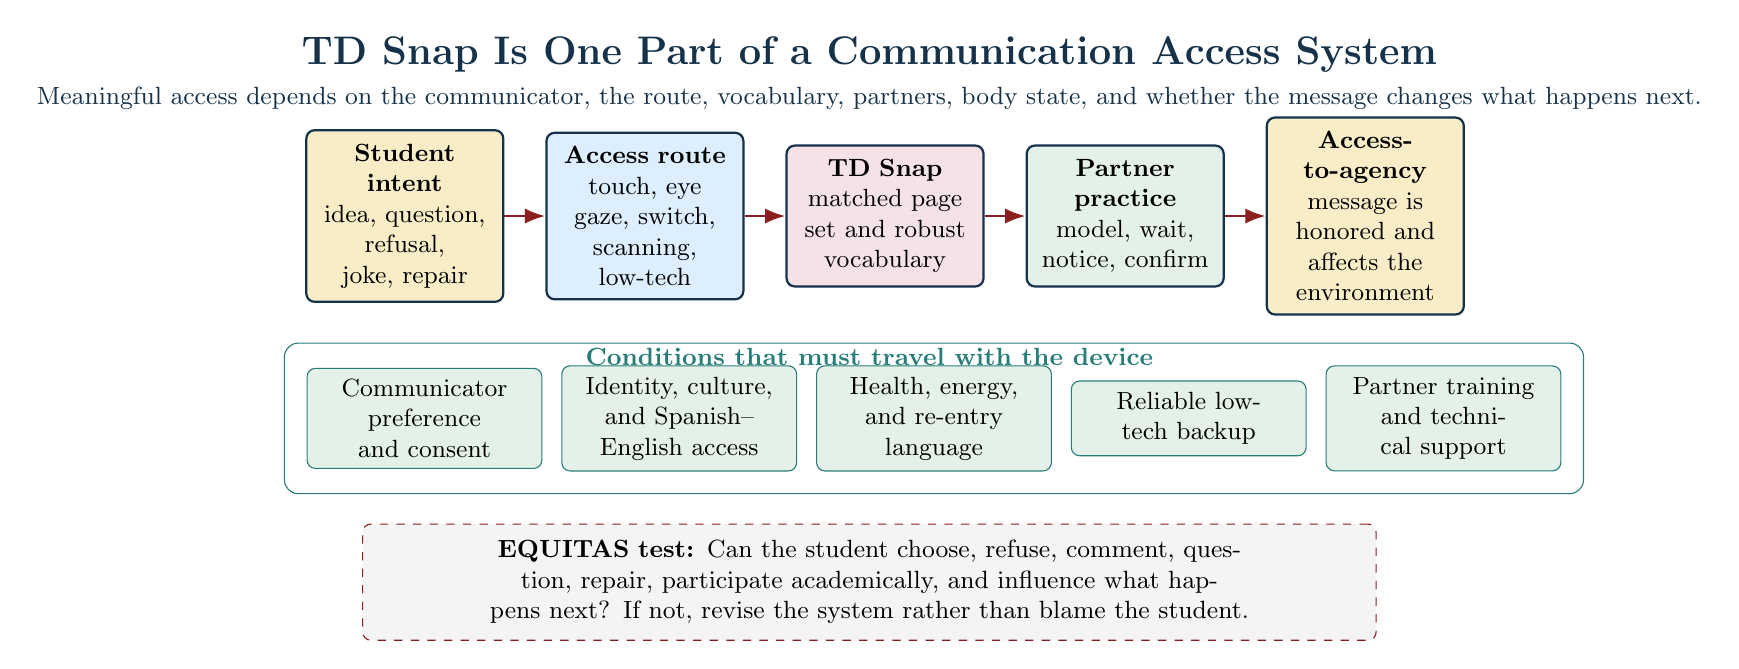
\begin{tikzpicture}[
  font=\sffamily,
  flowstep/.style={draw=DeepNavy, rounded corners=3pt, line width=0.8pt,
    text width=2.15cm, minimum height=1.55cm, align=center, inner sep=5pt, font=\small},
  support/.style={draw=MidTeal, rounded corners=3pt, fill=SoftGreen,
    text width=2.70cm, minimum height=0.90cm, align=center, inner sep=4pt, font=\small},
  flow/.style={-{Latex[length=2.6mm]}, line width=1pt, draw=PrimaryRed}
]

\node[font=\bfseries\Large, text=DeepNavy] (title) at (6.8,4.6)
  {TD Snap Is One Part of a Communication Access System};
\node[font=\small, text=DeepNavy, align=center] at (6.8,4.05)
  {Meaningful access depends on the communicator, the route, vocabulary, partners, body state, and whether the message changes what happens next.};

\node[flowstep, fill=SoftGold] (intent) at (0.9,2.55) {\textbf{Student intent}\\idea, question, refusal, joke, repair};
\node[flowstep, fill=SoftBlue, right=0.52cm of intent] (access) {\textbf{Access route}\\touch, eye gaze, switch, scanning, low-tech};
\node[flowstep, fill=SoftRose, right=0.52cm of access] (snap) {\textbf{TD Snap}\\matched page set and robust vocabulary};
\node[flowstep, fill=SoftGreen, right=0.52cm of snap] (partner) {\textbf{Partner practice}\\model, wait, notice, confirm};
\node[flowstep, fill=SoftGold, right=0.52cm of partner] (agency) {\textbf{Access-to-agency}\\message is honored and affects the environment};

\draw[flow] (intent) -- (access);
\draw[flow] (access) -- (snap);
\draw[flow] (snap) -- (partner);
\draw[flow] (partner) -- (agency);

\node[font=\bfseries\small, text=MidTeal] at (6.8,0.76) {Conditions that must travel with the device};
\node[support] (preference) at (1.15,-0.02) {Communicator preference and consent};
\node[support, right=0.24cm of preference] (identity) {Identity, culture, and Spanish--English access};
\node[support, right=0.24cm of identity] (health) {Health, energy, and re-entry language};
\node[support, right=0.24cm of health] (backup) {Reliable low-tech backup};
\node[support, right=0.24cm of backup] (training) {Partner training and technical support};

\node[draw=PrimaryRed, dashed, rounded corners=3pt, fill=SoftGray,
  text width=12.45cm, align=center, inner sep=6pt, at={(6.8,-2.10)},
  font=\small] (audit)
  {\textbf{EQUITAS test:} Can the student choose, refuse, comment, question, repair, participate academically, and influence what happens next? If not, revise the system rather than blame the student.};

\node[draw=MidTeal, rounded corners=5pt, fit=(preference)(identity)(health)(backup)(training),
  inner sep=8pt] {};

\end{tikzpicture}
\end{document}
